\documentclass[11pt]{article}
\usepackage[utf8]{inputenc}\usepackage[T1]{fontenc}
\usepackage{amsmath,amssymb,amsthm}\usepackage[margin=1in]{geometry}
\usepackage{graphicx}\usepackage{booktabs}
\usepackage[hidelinks]{hyperref}
\newcommand{\Adm}{\mathrm{Adm}}
\newtheorem{theorem}{Theorem}\newtheorem{definition}{Definition}

\title{The First-Principles Origin of the Tail Constant $K$ on the $6N$ Skeleton:\\
$K=\rho\cdot\mathrm{tail}_{\mathfrak S}(d)\cdot B$ and a Single Scale}
\author{Ruqing Chen\\
\small GUT Geoservice Inc., Montreal, Quebec, Canada\\
\small \texttt{ruqing@hotmail.com}}
\date{\today}

\begin{document}
\maketitle

\begin{abstract}
The closed-form right-centre survival of Part~VII,
$P(N{+}d\text{ twin}\mid\omega)=K\prod_{q\in\mathrm{POOL}}f_q(d,N)$ with
$\mathrm{POOL}=\{5,\dots,47\}$, carried one empirical constant $K\approx0.105$.
We give its first-principles origin. The constant factors as
\[
  K(d)=\rho\cdot\mathrm{tail}_{\mathfrak S}(d)\cdot B,
\]
where $\rho$ is the twin-centre line density (Part~VIII),
$\mathrm{tail}_{\mathfrak S}(d)=\mathfrak{S}(d)/\mathfrak{S}_{\mathrm{POOL}}(d)$
is the part of the Hardy--Littlewood singular series carried by primes $>47$, and
$B=\prod_{q\in\mathrm{POOL}}\mathfrak{S}_q(d)/\langle f_q\rangle$ is a pure
Chinese-Remainder basis-conversion constant, predicted analytically as
$B\simeq6.535$ and $d$-independent. Measured across $d$ on $S_9$ and $S_{10}$, the
ratio $K/(\rho\,\mathrm{tail}_{\mathfrak S})$ is constant to a coefficient of
variation of $0.31\%$ ($S_9$) and $0.16\%$ ($S_{10}$), and equals the predicted
$B$ to within $0.4\%$. $K$ is therefore not a free parameter. Moreover, since
Part~VIII gave the bridge constant $C_0=1/\rho$, both constants of the theory
reduce to the single scale $\rho$: the conditional gap preference $r(d\mid\omega)$
contains no fitted constant at all, only $\rho$ and closed-form
singular-series / CRT structure. No claim is made about the infinitude of twin
primes or any $k$-tuple conjecture.
\end{abstract}

\section{What $K$ absorbs}

Part~VII wrote the right-centre survival as $K\prod_{\mathrm{POOL}}f_q(d,N)$, a
product of pure CRT factors over $q\in\{5,\dots,47\}$ times a constant $K$
absorbing everything outside that finite product: the primes $q>47$, and the
conversion from the relative CRT product to an absolute probability. We show this
absorbed content is itself analytic.

The key is the merged-level identity of Part~VIII, $P_{\mathrm{merged}}(d)=
\rho\,\mathfrak{S}(d)$, where $\mathfrak{S}(d)=\prod_{q>3}\mathfrak{S}_q(d)$ is the
Hardy--Littlewood singular series and $\rho$ the twin-centre density. Comparing
with the Part~VII form averaged over $\omega$,
$P_{\mathrm{merged}}(d)=K\langle\prod_{\mathrm{POOL}}f_q\rangle$, gives
\[
  K=\frac{\rho\,\mathfrak{S}(d)}{\langle\prod_{\mathrm{POOL}}f_q\rangle_{\mathrm{merged}}}
   =\rho\cdot\underbrace{\frac{\mathfrak{S}(d)}{\mathfrak{S}_{\mathrm{POOL}}(d)}}_{\mathrm{tail}_{\mathfrak S}(d)}
    \cdot\underbrace{\frac{\mathfrak{S}_{\mathrm{POOL}}(d)}{\langle\prod_{\mathrm{POOL}}f_q\rangle}}_{B},
\]
since the merged average of the CRT product is the POOL part of the singular
series up to the basis factor $B$.

\begin{definition}[basis-conversion constant]
\[
  B=\prod_{q\in\mathrm{POOL}}\frac{\mathfrak{S}_q(d)}{\langle f_q\rangle_q},\qquad
  \langle f_q\rangle_q=\tfrac{1}{|\!\Adm_q|}\,[\,d\ q\text{-safe}\,]
   +\bigl(1-\tfrac{1}{|\!\Adm_q|}\bigr)f_q^{\nmid}(d),
\]
where $\Adm_q$ are the twin-admissible residues mod $q$ and $f_q^{\nmid}$ the
$q\nmid N$ admissible fraction. $B$ is the accumulated difference between the
singular-series single-prime factor and the CRT mean factor over the POOL primes;
it is closed-form and, as shown below, $d$-independent.
\end{definition}

\section{Confirmation on two shells}

\begin{theorem}[origin of $K$]\label{thm:K}
On $S_9$ and $S_{10}$, $K(d)=\rho\cdot\mathrm{tail}_{\mathfrak S}(d)\cdot B$ with
$B$ a $d$-independent constant equal to the CRT prediction $6.535$. The ratio
$K/(\rho\,\mathrm{tail}_{\mathfrak S})$ is constant to CV $0.31\%$ ($S_9$),
$0.16\%$ ($S_{10}$), matching $B$ to within $0.4\%$.
\end{theorem}

\begin{table}[h]\centering\small
\begin{tabular}{rcccc}
\toprule
$d$ & $K$ meas & $\rho\cdot\mathrm{tail}$ & $K/(\rho\,\mathrm{tail})$ & $/B_{\mathrm{CRT}}$\\
\midrule
\multicolumn{5}{l}{\emph{$S_{10}$ ($\rho=0.015992$, $B_{\mathrm{CRT}}=6.535$)}}\\
1  & 0.10276 & 0.01574 & 6.530 & 0.999\\
5  & 0.10323 & 0.01574 & 6.560 & 1.004\\
7  & 0.10326 & 0.01574 & 6.562 & 1.004\\
11 & 0.10294 & 0.01574 & 6.542 & 1.001\\
13 & 0.10293 & 0.01574 & 6.541 & 1.001\\
17 & 0.10306 & 0.01574 & 6.549 & 1.002\\
35 & 0.10523 & 0.01606 & 6.553 & 1.003\\
\midrule
\multicolumn{2}{l}{mean ($S_{10}$)} & & 6.548 & CV $0.16\%$\\
\multicolumn{2}{l}{mean ($S_9$)} & & 6.568 & CV $0.31\%$\\
\bottomrule
\end{tabular}
\caption{$K=\rho\cdot\mathrm{tail}_{\mathfrak S}(d)\cdot B$. The ratio
$K/(\rho\,\mathrm{tail})$ is $d$-independent and equals the CRT prediction $B=6.535$
to within $0.4\%$, on both shells.}
\label{tab:K}
\end{table}

\begin{figure}[h]\centering
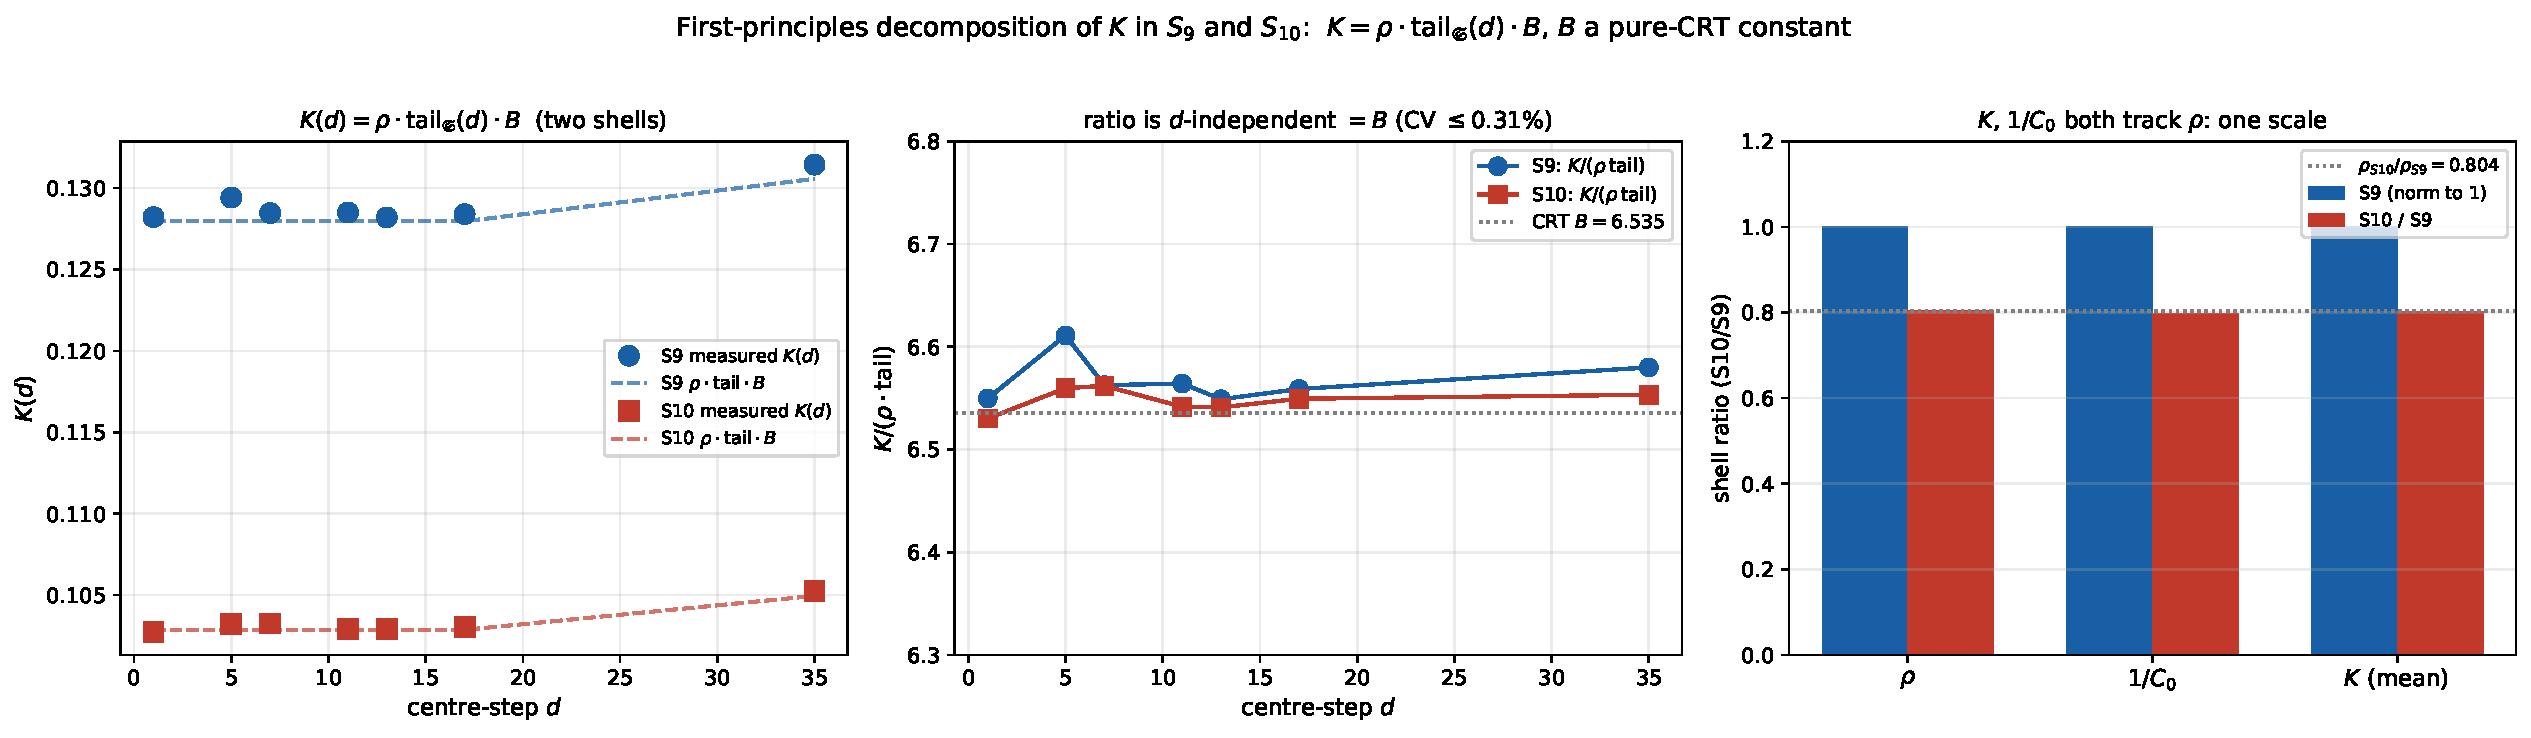
\includegraphics[width=\textwidth]{fig_paper11_K.pdf}
\caption{Left: $K(d)$ versus $\rho\,\mathrm{tail}_{\mathfrak S}(d)\,B$ on both
shells. Centre: the ratio $K/(\rho\,\mathrm{tail})$ is flat at the CRT constant
$B=6.535$. Right: $K$ and $1/C_0$ both scale from $S_9$ to $S_{10}$ as $\rho$
does (factor $0.80$), confirming $\rho$ is the single scale.}
\label{fig:K}
\end{figure}

The decisive evidence that the only scale is $\rho$: between $S_9$ and $S_{10}$
the density drops from $0.0199$ to $0.0160$ (factor $0.80$), and $K$ drops by the
same factor ($0.128\to0.103$) while $K/(\rho\,\mathrm{tail})$ stays at $6.55$.
The shell dependence of $K$ is entirely the shell dependence of $\rho$;
$\mathrm{tail}_{\mathfrak S}(d)$ and $B$ are shell-independent arithmetic.

\section{One scale for the whole theory}

Part~VIII gave $C_0=1/\rho$; this paper gives $K=\rho\,\mathrm{tail}_{\mathfrak
S}(d)\,B$. Both constants of the series reduce to the single density $\rho$. The
fully assembled conditional gap preference,
\[
  r(d\mid\omega)=\mathfrak{S}(d)\,\rho\,P(N{+}d\text{ twin}\mid\omega),\qquad
  P=K\!\prod_{\mathrm{POOL}}\! f_q=\rho\,\mathrm{tail}_{\mathfrak S}(d)\,B\!\prod_{\mathrm{POOL}}\! f_q,
\]
contains no fitted constant: $\mathfrak{S}$ and $\mathrm{tail}_{\mathfrak S}$ are
the Hardy--Littlewood singular series, $f_q$ and $B$ are closed-form CRT, and
$\rho$ is the twin-centre density (given, to leading order, by the
Hardy--Littlewood twin constant and the shell's mean $1/\ln^2$). The single
empirical input is $\rho$, and $\rho$ is itself a known density rather than a
constant of this construction.

\section{Conclusion}

The tail constant $K$ of Part~VII is not a free parameter. It decomposes as the
twin density $\rho$, the $>47$ tail of the Hardy--Littlewood singular series, and
a closed-form Chinese-Remainder basis constant $B\simeq6.535$, confirmed on two
shells to CV $\le0.31\%$ and matching the CRT value to $0.4\%$. With
$C_0=1/\rho$ from Part~VIII, the entire conditional theory rests on the single
scale $\rho$. The residual $0.2$--$0.4\%$ excess of the measured ratio over $B$ is
the uniform-residue approximation in the $q\nmid N$ branch, the same
few-tenths-of-a-percent effect seen throughout. As in every part of this series,
no claim is made about the infinitude of twin primes or any $k$-tuple conjecture;
this is a measured, closed-form, factor-resolved account of the conditional gap
structure of the $6N$ twin skeleton.

\paragraph{Data and code availability.}
The decomposition is openly available~\cite{repo}; the $S_{10}$ twin count
$23{,}988{,}173$ matches Part~I.

\begin{thebibliography}{9}
\bibitem{ChenI} R.~Chen, \emph{Prime distribution on the $6N$ skeleton} (Part~I),
Zenodo, doi:10.5281/zenodo.20470367 (2026).
\bibitem{ChenVII} R.~Chen, \emph{A closed form for the conditional twin-gap
distribution} (Part~VII), Zenodo, doi:10.5281/zenodo.20518470 (2026).
\bibitem{ChenVIII} R.~Chen, \emph{The arithmetic structure of the bridge
constant} (Part~VIII), Zenodo, doi:10.5281/zenodo.20519998 (2026).
\bibitem{HL} G.~H.~Hardy, J.~E.~Littlewood, \emph{Partitio Numerorum III}, Acta
Math.\ \textbf{44} (1923), 1--70.
\bibitem{repo} R.~Chen, \emph{$6N$ twin-prime tail constant: data and code},
\url{https://github.com/Ruqing1963/6N-twin-prime-tail-constant} (2026).
\end{thebibliography}

\end{document}
